\leavevmode\newline \leavevmode\newline
{\centering
\noindent{\Large \textbf{Learning a Language Like Infants do: Results and Challenges for Developmentally Inspired NLP}}\\  \vspace*{-0.1cm} \leavevmode\newline
{\normalsize \textbf{Emmanuel Dupoux}}\\
{\normalsize {École des Hautes Études en Sciences Sociales (EHESS), Paris, France}}\\


\begin{figure}[h!]
  \centering
      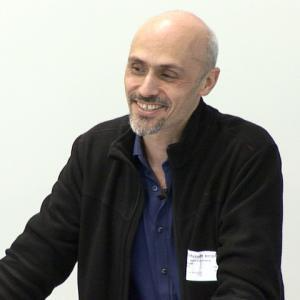
\includegraphics[width=0.15\linewidth]{invited_talks/emmanuel_dupoux_invited_1.png}
\end{figure}

 {\normalsize \textbf{Tuesday, Jan 21, 2025} -
 Room: \textbf{???} -
 Time: \textbf{09:30-10:30}\\\leavevmode\newline
 }
}

{\textbf{Abstract:}}
Instead of building AI systems that match human adults performance on tasks of interest, why not building an “AI child” that will be able to learn autonomously any task? This rather old idea has been notoriously difficult to implement, yet progress in machine learning and ecological datasets of parent- child interaction put us today in a good position to get a stab at it. We first describe the general conditions of autonomous language learning in the human child (continuous, scarce, noisy, multimodal, interactive data; fast, stable, overlapping learning curves), and propose methodological principles to compare child and machine learning abilities back to back. We then present some first results on (textless) speech language models showing a 3 to 5 orders of magnitude gap in sample efficiency (in favor of human children) and discuss competing hypotheses about what children have that current ai systems are lacking that could explain this large performance gap.\\

{\textbf{Bio:}}
Emmanuel Dupoux is a Professor of Cognitive Psychology at the École des Hautes Études en Sciences Sociales (EHESS) in Paris. He earned his Ph.D. in Cognitive Psychology from EHESS in 1989, focusing on the mechanisms and representations that enable infants to acquire language and become cognitively functional within their culture. His research expertise lies in cognitive development, psycholinguistics, language acquisition, cognitive modeling, and machine learning. He specializes in studying early language acquisition, phonological ‘deafnesses’ in speech perception, and the development of social cognition. He also investigates how machine learning and artificial intelligence can provide quantitative models of processing and learning in infants. Throughout his career, he has received several awards and honors, including an Advanced ERC grant and the organization of the Zero Resource Speech Challenge (2015, 2017, 2019) and the Intuitive Physics Benchmark (2019).\\

\clearpage